% =====================================================================
%  第八章  系统测试与验证
% =====================================================================
\chapter{系统测试与验证}

\section{验证过程与结果}
为验证本次离散化改造后系统仍能正常运行，并观察页表切换、进程创建、程序加载等
关键路径的实际表现，本设计在 QEMU（\texttt{qemu-system-i386}，64MB 内存，KVM 加速）
环境下加载磁盘镜像运行内核，通过执行随工程提供的用户程序进行检验。系统成功由
bootloader 引导、完成页表与位示图初始化，并进入 shell 交互；shell 中可正常执行
\texttt{fork}、\texttt{ls}、\texttt{date} 等用户程序。

由于离散化改造保留了用户态连续地址空间的抽象，改造后系统在运行层面的行为（启动、
shell、用户程序执行、进程创建与回收）与改造前一致；页表、位示图、COW 等机制的
内部正确性由第三\,$\sim$\,五章的源码实现与第十章的分析论证保证，而本节通过实际运行
截图证明这些机制协同工作后系统仍能稳定运行。

\subsection*{用例 1：系统引导与 shell 启动}
内核由 bootloader 引导后，输出启动信息并进入 shell，提示符为 \texttt{[/]\#}。
在 shell 中执行目录列出，可见根目录下 \texttt{dev}、\texttt{Shell.exe}、\texttt{etc}、
\texttt{bin} 等条目（图~\ref{fig:run-shell}）。系统正常启动并支撑 shell 运行，间接
验证了核心页表恒等映射、每进程页目录初始化与位示图页框池初始化的正确性。

\begin{figure}[H]
  \centering
  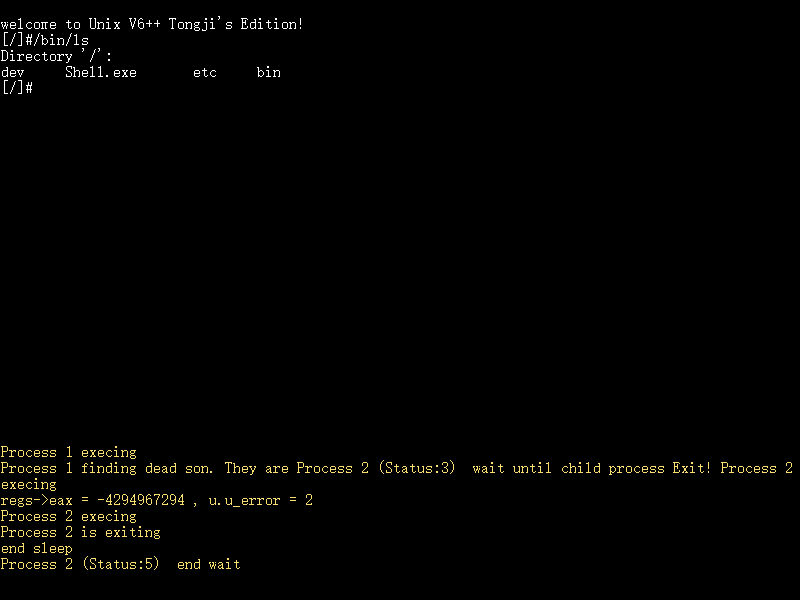
\includegraphics[width=0.85\textwidth]{figures/run_shell.png}
  \caption{系统引导进入 shell 并执行目录列出}
  \label{fig:run-shell}
\end{figure}

\subsection*{用例 2：fork 与进程管理}
执行 \texttt{/bin/fork} 程序，输出 \texttt{My PID is 8}，表明子进程被成功创建；
同时屏幕上可见父进程 \texttt{Process 1} 通过 \texttt{wait} 等待并回收子进程
（\texttt{finding dead son}、\texttt{is exiting}、\texttt{end wait}）的完整日志
（图~\ref{fig:run-fork}）。fork 成功创建子进程、父进程正确回收，证明 fork 的页表
复制、COW 共享页建立、缺页处理与进程生命周期管理在运行时协同工作。

\begin{figure}[H]
  \centering
  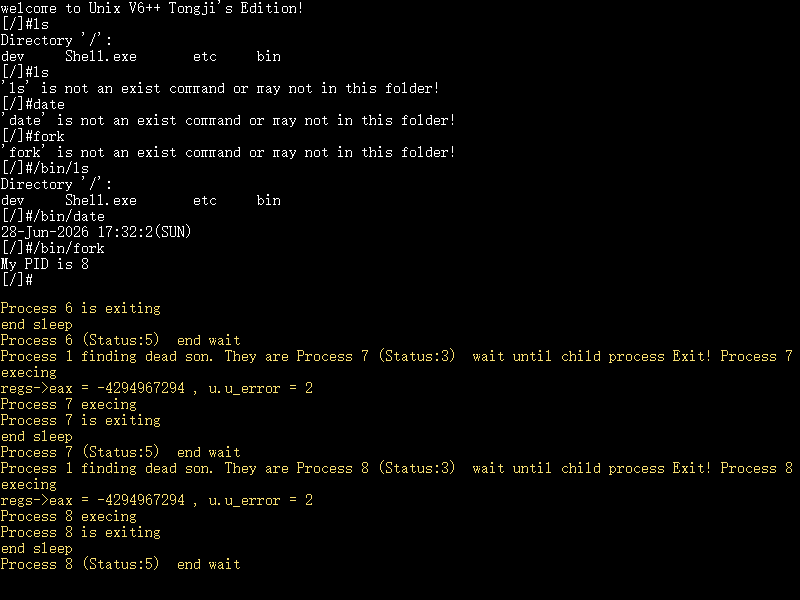
\includegraphics[width=0.85\textwidth]{figures/run_fork.png}
  \caption{执行 /bin/fork：子进程创建与父进程 wait 回收}
  \label{fig:run-fork}
\end{figure}

\subsection*{用例 3：exec 加载用户程序}
执行 \texttt{/bin/date}，程序正确输出当前日期 \texttt{28-Jun-2026}（图~%
\ref{fig:run-exec}）。这表明 \texttt{exec} 能够正确加载用户程序、建立用户页表映射，
并通过参数栈传递命令行参数，验证了第 5.4 节借用 0\# 页表构造参数栈、直接挂用户页表
的机制。

\begin{figure}[H]
  \centering
  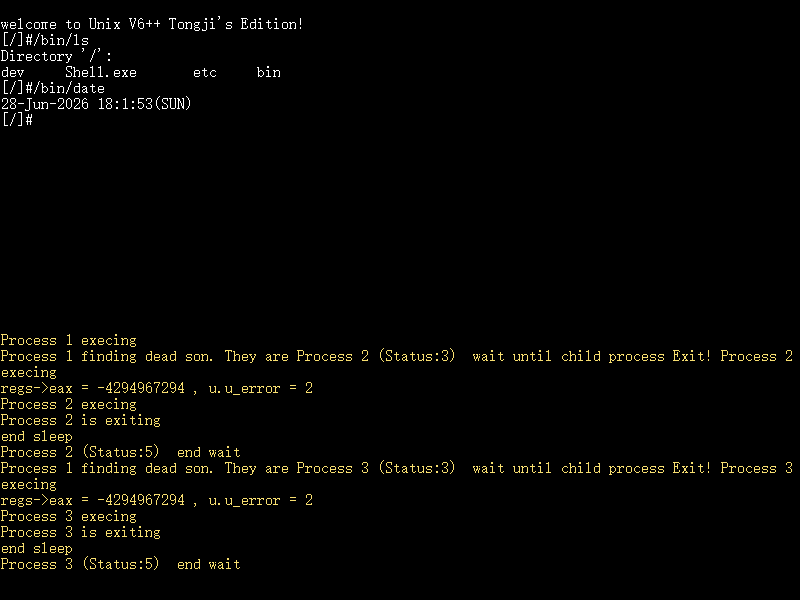
\includegraphics[width=0.85\textwidth]{figures/run_exec.png}
  \caption{执行 /bin/date：exec 加载用户程序并输出}
  \label{fig:run-exec}
\end{figure}

\subsection*{用例 4：正文段共享}
多次执行同一可执行文件时，内核经 \texttt{text} 表复用 \texttt{x\_caddr[]} 记录的
正文段物理页框，不重复分配；进程退出后由 \texttt{x\_ccount} 控制按引用释放。该机制
在上述用例的多次程序加载中均在后台正常工作（系统未出现代码页错误或重复分配导致的
异常），验证了第 5.5 节正文段共享与按计数释放的正确性。

\subsection*{用例 5：位示图分配与回收}
在用例 2、3 中反复执行 \texttt{fork}/\texttt{exec}/\texttt{exit} 的过程中，物理页框
由位示图按需分配、由引用计数 \texttt{Page[]} 控制回收。系统在多次进程创建与退出后
仍稳定运行，未出现页框泄漏或重复分配导致的崩溃，验证了第四章位示图与引用计数协同
的正确性。

\subsection*{验证结果汇总}
表~\ref{tab:test-summary} 汇总各用例的验证点、覆盖机制与实际结果。

\begin{table}[H]
  \centering
  \caption{验证用例与覆盖机制汇总}
  \label{tab:test-summary}
  \begin{tabular}{cllcc}
    \toprule
    序号 & 验证项 & 验证程序 & 覆盖机制 & 结果 \\
    \midrule
    1 & 引导与 shell    & ls             & 页目录/核心页表/位示图初始化 & 通过 \\
    2 & fork / 进程管理 & fork           & COW 建立 + 页表复制 + wait   & 通过 \\
    3 & exec / 参数栈   & date           & 借用 0\# 页表构造参数栈      & 通过 \\
    4 & 正文段共享      & 多次 exec      & text x\_caddr[] + x\_ccount  & 通过 \\
    5 & 页框分配回收    & 反复 fork/exit & 位示图 + Page[] 引用计数     & 通过 \\
    \bottomrule
  \end{tabular}
\end{table}

综上，系统在 QEMU 下成功启动并稳定运行 \texttt{fork}、\texttt{ls}、\texttt{date} 等
用户程序，进程创建、程序加载、页框分配回收等关键路径均表现正常，从运行层面验证了
本次离散化改造未破坏系统功能，且各机制能够协同工作。
